%%%%%%   TIPO DE DOCUMEN%TO: Reporte   %%%%%%
\documentclass[letterpaper,11pt]{report}
%%%%%%%%%%%%%%%%%%%%%%%%%%%%%%%%%%%%%%%%%%%%

%%%%%%%   PAQUETES   %%%%%%%
\usepackage[spanish]{babel}
\usepackage{graphicx}
\usepackage[utf8]{inputenc}
\usepackage{float}
%%%%%%%%%%%%%%%%%%%%%%%%%%%%

%%%%%%%%%%%%%%%%%%%%%%%%%%%%%%%%%%%%%%%%
%%%%%%%   INICIO DEL DOCUMENTO   %%%%%%%
%%%%%%%%%%%%%%%%%%%%%%%%%%%%%%%%%%%%%%%%
\begin{document}

    %%%%%%% Renombrar en espaNol %%%%%%
    \renewcommand{\tablename}{Tabla} %Escribe Tabla en lugar de Cuadro
    \renewcommand{\listtablename}{\'Indice de tablas} %Escribe Indeice de tablas en lugar de Indice de cuadros

    %%%%%%%   PORTADA   y RESUMEN   %%%%%%% Este es el contenido agregado de la secci\'on 2.

    %%%%%%%%%%%%%%%%%%%%%%%%%%%%%
%%%%%      PORTADA      %%%%%
%%%%%%%%%%%%%%%%%%%%%%%%%%%%%

\begin{titlepage}

    \centering %Todo centrado

    %%%%  LOGO DE LA ESCUELA   %%%%
    
\includegraphics[scale=0.17]{imagenes/escom-ipn} %Imagen para portada
    %%%%  NOMBRE DE LA ESCUELA   %%%%
    \LARGE{\\ Instituto Polit\'ecnico Nacional}
    \LARGE{\\ Escuela Superior de C\'omputo}
    
    \vspace{1cm} %Espacio vertical

    %%%%  TITULO Y NÚMERO DE TRABAJO   %%%%
    \LARGE \textbf{ Nombre del Trabajo Terminal}
    \LARGE {\\ Número de Trabajo Terminal}

    \vspace{1cm} %Espacio vertical

    \LARGE \textit{Que para cumplir con la opción de titulación curricular en la carrera de:}
    \LARGE \textbf{\\ Ingeniería en Sistemas Computacionales}

    \vspace{1cm} %Espacio vertical

    %%%%   ALUMNOS   %%%%
   \textit{Presentan}\\
    Alumno 1 \\
    Alumno 2 \\
    Alumno 3

    \vspace{1cm} %Espacio vertical

    %%%%   Directores   %%%%
   \textit{Directores}\\
    M. en C. José David Ortega Pacheco \bigskip  Director 2

\end{titlepage} %incluye el archivo portada.tex
    %%%%%%%%%%%%%%%%%%%%%%%
%%%%    RESUMEN    %%%%
%%%%%%%%%%%%%%%%%%%%%%%

\begin{abstract}

  Aquí va el resumen general del documento de trabajo terminal.

\end{abstract}
 %Incluir resumen del documento (resumen.tex)
	%%%%%%%%%%%%%%%%%%%%%%%
%%%%  ADVERTENCIA  %%%%
%%%%%%%%%%%%%%%%%%%%%%%

\begin{small}
	
	\centering \textbf{Advertencia} 
	
\end{small}


	\textit{“Este documento contiene información desarrollada por la Escuela
		Superior de Cómputo del Instituto Politécnico Nacional, a partir de datos y
		documentos con derecho de propiedad y por lo tanto, su uso quedará
		restringido a las aplicaciones que explícitamente se convengan.”} \\
	
		La aplicación no convenida exime a la escuela su responsabilidad técnica y
		da lugar a las consecuencias legales que para tal efecto se determinen. \\
		
		Información adicional sobre este reporte técnico podrá obtenerse en: \\
		
		La Subdirección Académica de la Escuela Superior de Cómputo del Instituto
		Politécnico Nacional, situada en Av. Juan de Dios Bátiz s/n Teléfono:
		57296000, extensión 52000.
		






		 %Incluir advertencia del archivo (advertencia.tex)
    %%%%%%%   INCLUIR ENCABEZADOS EN INDICES Y CAPITULOS   %%%%%%%
    \pagestyle{headings}

    %%%%%%%   NUMERACION EN CONTENIDO E INDICE DE TABLAS Y FIGURAS   %%%%%%%
    \pagenumbering{roman} %NUmeros romanos
    %\setcounter{page}{1} %Comienza en I por default, aquI se puedo modificar

    %%%%%%   INCLUIR CONTENIDO, INDICE DE FIGURAS E INDICE DE TABLAS   %%%%%%
    \tableofcontents
    \listoffigures
    \listoftables

    %%%%%%%   NUMERACION EN CAPITULOS   %%%%%%%
    \clearpage %Para iniciar con los arAbigos
    \pagenumbering{arabic} %Numeros arabigos
    %\setcounter{page}{1} %Comienza en 1 por default, aquI se puede modificar

    %%%%%%%   INCLUYE CAPITULOS Y SECCIONES   %%%%%%%
    \chapter{Introducci\'on}

La Clasificación Internacional del Funcionamiento de la Discapacidad y de la Salud (CIF) define la discapacidad como un término genérico que engloba deficiencias, limitaciones de actividad y restricciones para la participación social. La discapacidad forma parte de la condición humana: “… casi todas las personas sufrirán algún tipo de discapacidad transitoria o permanente en algún momento de su vida, y las que lleguen a la senilidad experimentarán dificultades crecientes de funcionamiento”. \\

De acuerdo a los informes de la Organización Mundial de la Salud (OMS), se estima que más de mil millones de personas viven con algún tipo de discapacidad; es decir, alrededor del 15\% de la población mundial (según las estimaciones de la población mundial en 2010) \cite{uno}. En relación con lo anterior, en el país existen 31.5 millones de hogares, de ellos 6.1 millones reportan que existe al menos una persona con discapacidad; es decir, en 19 de cada 100 hogares vive una persona que presenta alguna dificultad. \\

En el 2013 6.6\% de la población mexicana reportó tener una discapacidad, siendo en su mayoría las personas adultos mayores, con 51.4\%, informó el Instituto Nacional de Estadística y Geografía (INEGI). Por otra parte, la Encuesta Nacional de Ingresos y Gastos de los Hogares 2012 (ENIGH 2012), dicho porcentaje de la población del país presentó dificultad (discapacidad) para realizar al menos una de las actividades como: caminar, ver, escuchar, hablar o comunicarse, poner atención o aprender, atender el cuidado personal y mental \cite{dos}. Mientras que en los adultos mayores la enfermedad y la edad es el factor detonante. En los adultos mayores, el 50.9\% de las discapacidades se tienen por origen de la edad avanzada. \\
De acuerdo con las proyecciones del Consejo Nacional de Población (CONAPO), hasta 2010 la población en el Distrito Federal de 65 años en adelante representa el 7.9\% del total. Para 2030, serán los “viejitos” del futuro y demandarán productos y servicios especiales para ellos. \\

Aunado a este factor, "las Instituciones del Gobierno y la oferta de salud entre hospitales y personal especializado no son suficientes para atender a la población que sufre de alguna discapacidad, por otra parte del costo por estos servicios es elevado oscilando desde \$7,000 M.N. a \$30,000 M.N. mensuales \cite{tres}. \\

En la actualidad existen programas sociales por parte del Gobierno de la Ciudad de México, uno de ellos es “Médico en tu casa” este programa fue creado para reducir índices de mortalidad por embarazos en Iztapalapa y Gustavo A. Madero. El cual consiste en enviar médicos para que atiendan a mujeres embarazadas, adultos mayores y niños. El principal objetivo de este programa es brindar atención a la población vulnerable, principalmente adultos mayores, discapacitados, enfermos terminales, así como disminuir el índice de mortalidad materna-infantil en la capital. \\

Sumado a lo anterior es necesario utilizar herramientas que nos permitan facilitar el cuidado de las personas con discapacidad, dando una opción más accesible para la población que no cuente con recursos necesarios para pagar algún servicio de cuidado y atención. \\

La idea de utilizar este tipo de herramientas es facilitar el cuidado y la atención de las personas con alguna discapacidad, teniendo en cuenta que aún pueden realizar actividades de la vida cotidiana, además de estar pendientes de los momentos exactos en los que la persona presente una situación delicada en su estado de salud. Una de estas alternativas es utilizar sensores que permitan supervisar las vulnerabilidades que presente, buscando aprovechar al máximo el tiempo de los familiares sin descuidar la atención que requiere el familiar con discapacidad, sin dejar de lado la necesidad de reducir los precios que conlleva el cuidado de las personas con discapacidad, ya que con esta propuesta permitirá a los familiares que no cuenten con los recursos para este tipo de servicios, puedan usarla como apoyo al cuidado de sus familiares, siendo el costo del prototipo más accesible, pensando en que se realice con un menor monto al requerido por las instituciones que brindan estos servicios. \\




	   \section{Contexto de trabajo}

Se describe el área donde se esta trabajando y en qué contexto
	   \section{Problemática}

   
	   \section{Trabajo previo}

  
	   \section{Justificación}

Como se mencionó anteriormente la discapacidad en el país ha ido en aumento en los últimos años debido a la transición demográfica, la reducción de mortalidad-natalidad y accidentes ocasionados en el trabajo. La mayor parte de la población discapacitada son los adultos mayores de 60 años. Es decir, la enfermedad o la edad avanzada son las principales causas para todos los tipos de discapacidad considerados. Con el desarrollo de este prototipo se pretende dar atención a una necesidad social que cada vez va en aumento, debido a los altos costos que implica contratar un servicio especializado que aún no se encuentra plenamente desarrollado. Aunque es necesario puntualizar que este prototipo solo supervisará aquellos casos en los que el adulto mayor no se encuentre postrado en una cama. \\


\begin{table}[htb]
	\centering
	\begin{tabular}{|p{4cm}|p{1.5cm}|p{1.5cm}|p{1.5cm}|p{1.5cm}|}
		\hline
		Tipos de discapacidad & \multicolumn{4}{c|}{Grupos de edad} \\
		\cline{2-5} 
		& 0 a 14 años & 15 a 29 años & 30 a 59 años & 60 años o más \\
		\hline \hline
		Caminar, subir o bajar usando sus piernas. & 36.2 & 32.1 & 56.2 & 81.3 \\ \cline{2-5}
		\hline 
		Ver (aunque usen lentes). & 26.9 & 44.6	& 58.2 & 67.2 \\ \cline{2-5}
		\hline 
		Mover o usar sus brazos o manos. & 14.1 & 18.2 & 28.5 &	42.7 \\ \cline{2-5}
		\hline 
		Aprender, recordar o concentrarse. & 40.8 & 31.5 & 32.1 & 44.6 \\ \cline{2-5}
		\hline 
		Escuchar (aunque usen aparato auditivo). & 13.4	& 18.5 & 24.2 & 46.9 \\ \cline{2-5}
		\hline 
		Bañarse, vestirse o comer. & 37.4 & 16.4 & 14.5 & 29.3 \\ \cline{2-5}
		\hline 
		Hablar o comunicarse. & 45.6 & 28.5 & 13.4 & 14.0 \\ \cline{2-5}
		\hline 
		Problemas emocionales o mentales. & 26.6 & 28.0 & 20.1 & 16.3  \\ \cline{2-5}
		\hline
	\end{tabular}
	\textbf{\caption{\small{\textbf{Porcentaje de población con discapacidad, por tipo de discapacidad según grupos de edad en 2014 \cite{diez}.}}}}
	\label{Justificacion:Tabla1.1}
\end{table}

Por lo que se requiere de servicios especializados en salud enfocados a este sector, en la actualidad existen programas para atender este tipo de problemáticas por mencionar algunos provenientes del Gobierno de la Ciudad de México como: 

\begin{itemize}
	\item Médico en tu casa.
	\item Programa Nacional para el Desarrollo y la Inclusión de las personas con discapacidad.
\end{itemize}

Por parte de la iniciativa Privada existen servicios para este tipo de necesidad como:

\begin{itemize}
	\item Cuidado personalizado (Homewatch Care Givers).
	\item Estancia (La Casa de Las Lunas).
\end{itemize}

Teniendo costos elevados que desequilibran la economía familiar, tal y como se mencionó en la introducción de la investigación. Sin embargo, los programas gubernamentales no logran cubrir la demanda para estos servicios y por parte de la iniciativa privada sus costos son elevados, como consecuencia no toda la población cuenta con los recursos suficientes para pagar un servicio como esté. \\
 
Por lo que se propone un prototipo para ayudar a personas con determinada discapacidad, implementando una serie de alertas que permitan a los familiares estar al tanto de la situación del discapacitado, por otro lado, se busca que este prototipo sea portable y económico, de esta manera reducir los costos que significa este tipo de cuidados, siendo una alternativa o complemento de los servicios ya existentes. \\

Para cubrir la necesidad de la población con bajos recursos, se piensa diseñar una tarjeta de propósito específico a partir de sensores y microcontroladores adecuados con el fin de reducir los costos, ya que estos son muy accesibles en el mercado, utilizados para múltiples aplicaciones permitiendo que el prototipo sea escalable y portable. \\

Entre las diferencias con respecto a lo ya existente, son las alertas instantáneas emitidas por los sensores logrando mantener al familiar informado de la situación en la que se encuentra la persona con discapacidad. Cabe mencionar que los sistemas de monitoreo existentes están diseñados para que una persona esté siempre monitoreando la situación del discapacitado.


 
	   \section{Marco Teórico}

A continuación se presentan las variables que consideramos importantes para el desarrollo del proyecto, antes de llevar a cabo la elección de los dispositivos a emplear, previamente se elaboró una investigación de los signos vitales más indispensables del ser humano, por lo que para fines del proyecto y de acuerdo con lo analizado las variables a medir son la temperatura, considerando que es el primer parámetro para determinar una enfermedad, la segunda variable es un acelerómetro que por causa del envejecimiento de las personas suelen ser más predispuestas a sufrir alguna caída y por último la frecuencia cardíaca, esta última involucra un órgano muy importante para las personas por ello consideramos evaluar conjuntamente esta medida. Existen otras variables importantes pero por la complejidad para medirlas no entran en la posibilidad de incluirlas en este trabajo terminal, dichas variables pueden ser por ejemplo: la presión arterial, la glucosa, por mencionar algunas, ya que al medirlas no utilizan un método invasivo y no causan molestia al usuario. 

\subsection{Variables a medir}

En este apartado se muestra una descripción de las variables que elegimos y la importancia de cada una, de igual forma se explicaran los motivos por los que fueron seleccionadas. A continuación se en listan las variables seleccionadas y las cuales serán monitoreadas en este proyecto:

\begin{enumerate}
	\item Temperatura.
	\item Caídas.
	\item Frecuencia Cardíaca.
\end{enumerate}

\begin{enumerate}
	\item \textbf{Temperatura} 
	
	Se ha considero medir la temperatura corporal, está variable es de gran importancia para determinar las condiciones en las que se encuentra el enfermo, la constante medición de esta permite a enfermeros(as) y algún otro personal médico conocer la mejoría y situación del paciente, en algunos casos la temperatura se toma como primer parámetro para diagnosticar una enfermedad. \\
	
	La Secretaria de Salud establece que la temperatura corporal aceptable oscila entre los $36.5^{\circ}$C $47^{\circ}$C y los $37.2^{\circ}$C, mientras que las temperaturas fuera de este rango se consideran anormales, a continuación, se muestran los términos utilizados considerados anormales conforme a la Norma Oficial Mexicana NOM-031-SSA2-1999, considerando que no interviene un mecanismo termorregulador o se presenta un golpe de calor.
	
	\begin{itemize}
		\item \textbf{Fiebre:} La elevación anormal de la temperatura corporal por encima de los $38^{\circ}$C.
		\item \textbf{Hipertermia:} Es el estado de incremento de la temperatura del cuerpo que sobrepasa los $40^{\circ}$C.
		\item \textbf{Hipotermia:} En este estado la temperatura corporal se encuentra por debajo de los $36^{\circ}$C.
	\end{itemize}
	
	Por esta razón es importante tener controlada la temperatura en el rango que se considera aceptable. Nuestro cuerpo tiene mecanismos que regulan la temperatura y con el paso de los años se van perdiendo. Por esta importancia se decidió tomar la temperatura como una de las variables a medir en este proyecto \cite{once}.
	
	\item \textbf{Caídas}
	
	Las caídas son consideradas de alta importancia, debido las consecuencias que conllevan y pueden sufrir las personas de la tercera edad. Los tipos de caídas en adultos mayores pueden ser las siguientes:
	
	\begin{itemize}
		\item \textbf{Caída accidental:} Es aquella que generalmente se produce por una causa ajena al adulto mayor sano (ejemplo: tropiezo) y que no vuelve a repetirse.
		\item \textbf{Caída repetida:} Expresa la persistencia de factores predisponentes como, enfermedades crónicas múltiples, fármacos, pérdidas sensoriales, etc.
		\item \textbf{Caída prolongada:} Es aquella en la que el adulto mayor permanece en el suelo por más de 15 o 20 minutos por incapacidad de levantarse sin ayuda.	Los adultos mayores que tienen mayor prevalencia de caídas prolongadas son: aquellos de 80 años o más, con debilidad de miembros, con dificultades para las actividades cotidianas y aquellos que toman medicación \cite{doce}.
	\end{itemize}

	\begin{itemize}
		\item Escenarios y posturas de una persona al sufrir una caída.
		Para entender los escenarios y posturas se realizó un estudio con 240 personas de la tercera edad para monitorear sus actividades cotidianas (como: sentarse en una silla, sentarse en un inodoro, salir o entrar de un auto, sentarse o recostarse sobre la cama y caminar), a estas personas se les coloca un acelerómetro en diferentes partes del cuerpo, el cual detecta las señales tanto de las actividades mencionadas, como de alguna caída (caídas hacia delante o atrás, caídas laterales a la izquierda o derecha y caídas con las piernas rectas o flexionadas) que lleguen a sufrir los sujetos de estudio \cite{trece}. \\
		 
		En la figura 1.3 se detectaron los umbrales superior e inferior de caídas, donde se observa que estas tienen una señal con un pico muy alargado el cual está en un rango de aceleración de entre 0 y 7 g, a diferencia de la señal de las actividades cotidianas que no rebasan 1.5 g. \\
		
		\begin{figure}[h]
			\centering
			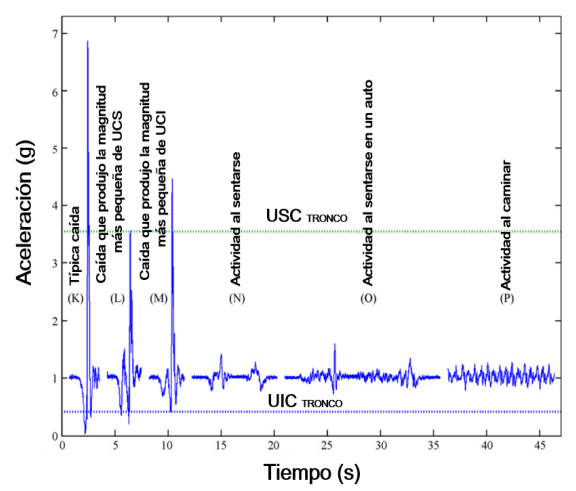
\includegraphics[scale=0.35]{introduccion/imagenes/grafica1_3}
			\textbf{\caption{\small{Representación de una señal para caídas y actividades cotidianas, en personas de la tercera edad usando un acelerómetro \cite{trece}.}}}
			\label{Seccion1.5.1:Figura1.3}
		\end{figure}
		
		En la figura 1.4 se muestran detalladamente los puntos de interés en la señal y cada una de las posiciones en las que se encontraba el adulto mayor al sufrir una caída, de igual manera se muestran detalladamente las actividades cotidianas realizadas en donde el acelerómetro registro actividad con pequeñas variaciones y similitudes, mostrando los puntos de interés en dicha señal.  \\
		
		\begin{figure}[h]
			\centering
			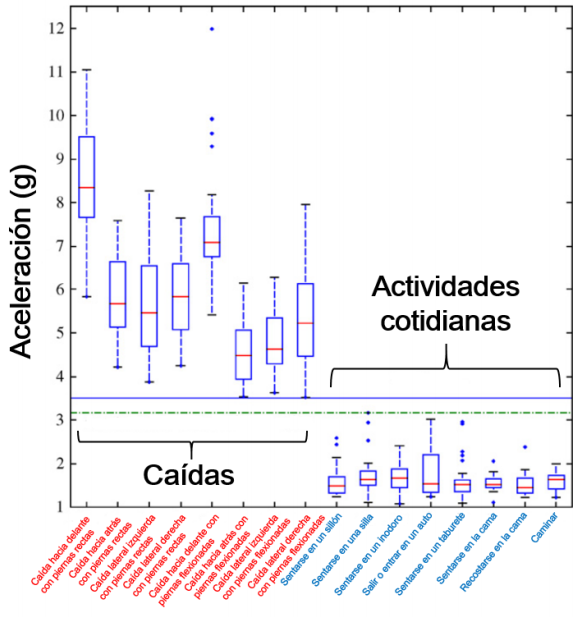
\includegraphics[scale=0.35]{introduccion/imagenes/grafica1_4}
			\textbf{\caption{\small{Puntos de interés en la señal que muestra: (a) posturas al sufrir una caída y (b) actividades cotidianas \cite{trece}.}}}
			\label{Seccion1.5.1:Figura1.4}
		\end{figure}
		
		Con base en las figuras 1.3 y 1.4 se establecen los escenarios en los que una persona puede sufrir algún tipo de caída y en donde se utilizan sensores acelerómetros en diferentes partes del cuerpo para realizar un muestreo de la aceleración. \\
		
		\begin{table}
%			\centering
			\resizebox*{12.5cm}{8cm}{
				\begin{tabular}{|l|c|c|c|}
					\hline
					Escenario & Postura	& Muestreo del acelerómetro & Caída \\
					\hline \hline
					Caída hacia adelante con piernas rectas	& De pie o recostado & 7.5g a 9.5g & Si \\
					\hline
					Caída hacia atrás con piernas rectas & De pie o recostado & 5g a 6.5g & Si \\
					\hline
					Caída lateral izquierda con piernas rectas & De pie o recostado & 4.5g a 6.5g & Si \\
					\hline
					Caída lateral derecha con piernas rectas & De pie o recostado & 5g a 6.5g & Si \\
					\hline
					Caída hacia adelante con piernas flexionadas & Sentado o inclinado & 6.8g a 7.8g & Si \\
					\hline
					Caída hacia atrás con piernas flexionadas & Sentado o inclinado & 4g a 5g & Si \\
					\hline
					Caída lateral izquierda con piernas flexionadas & Sentado o inclinado & 4.5g a 5.5g & Si \\
					\hline
					Caída lateral derecha con piernas flexionadas & Sentado o inclinado & 4.8g a 6g	& Si \\
					\hline
					Sentarse en un sillón & Sentado	& 1.2g a 1.8g & No \\
					\hline
					Sentarse en una silla & Sentado & 1.5g a 1.9g &	No \\
					\hline
					Sentarse en un inodoro & Sentado & 1.5g a 2g & No \\
					\hline
					Salir o entrar de un auto & Sentado o de pie & 1.2g a 2.5g & No \\
					\hline
					Sentarse en un taburete & Sentado & 1.2g a 1.5g & No \\
					\hline
					Sentarse en la cama	& Sentado & 1.4g a 1.6g & No \\
					\hline
					Recostarse en la cama & Recostado & 1.2g a 1.6g & No \\
					\hline
					Caminar & De pie & 1.5g a 1.8 & No \\
					\hline
				\end{tabular}
			}
		\textbf{\caption{\small{\textbf{Escenarios y posturas en los que el acelerómetro realizará muestreo.}}}}
		\end{table}
	
	 Por lo anterior y debido a la complejidad de detectar todos los escenarios de caídas, en este proyecto únicamente se detectará la caída típica, que es la caída hacia delante con las piernas rectas.
	\end{itemize}

	\item \textbf{Frecuencia Cardíaca}
	
	Esta variable es considerada importante puesto que involucra uno de los signos más relevantes para el óptimo funcionamiento del corazón, de modo que es el principal órgano del ser humano que nos mantiene con vida, por lo cual estimaremos dicha variable para este proyecto. \\
	
	El funcionamiento del corazón se manifiesta, al actuar como bomba impulsora, lo que determina el gasto cardíaco (cantidad de sangre enviada por el corazón al torrente circulatorio en un minuto), que representa el volumen de eyección sistólico en cada latido por minuto. La frecuencia cardíaca (FC) es un parámetro indicativo de la eficiencia con la que el corazón trabaja. En esfuerzos de tipo máximo se busca alcanzar la frecuencia cardíaca máxima para cada sujeto, sin pasar los límites que representen riesgo de provocar una falla o insuficiencia cardíaca durante la ejecución de un esfuerzo físico intenso. Para determinarla existen varios modelos matemáticos, pero el más común consiste en tomar la cifra de 220 y restarle la edad del sujeto. \\
	
	Por otro lado, habitualmente la tensión arterial se incrementa con la edad, más la sistólica que la diastólica, así como la presión del pulso (diferencia entre ambas), en las personas mayores de 65 años, el 40\% sufre de hipertensión arterial, y de ellos el 65\% - 70\% tienen riesgo de sufrir accidentes cardiovasculares, fatales o no. \\
	
	Con el paso de los años, el organismo pierde su habilidad para redistribuir el flujo sanguíneo desde las vísceras a los músculos en acción, de tal forma que la diferencia arteriovenosa de oxígeno (Dif a/v O2) medida en el músculo y la del flujo de retorno venoso al corazón durante el esfuerzo físico, es menor en las personas adultas mayores y sedentarias, con lo cual disminuye la reserva funcional \cite{catorce}. \\
	
	Algunos estudios realizados en poblaciones sanas, así como en pacientes hipertensos, con cardiopatía isquémica o con insuficiencia cardíaca, demuestran una asociación entre la FC elevada y un mayor riesgo de mortalidad. Según esto, cuanto mayor es la FC, menor es la expectativa de vida. La frecuencia cardíaca (FC) en reposo oscila entre 50 y 100 latidos por minuto en las personas adultas. Al nacer, la FC es más elevada porque el bebé la necesita para su adecuado crecimiento. A partir del primer mes de vida, la FC va disminuyendo hasta alcanzar las cifras normales de un adulto. El ejercicio físico o las situaciones de estrés provocan un aumento de la FC (taquicardia sinusal), que se considera normal \cite{quince}.
	
\end{enumerate}

\subsection{Sensores}

A continuación, se muestran algunas definiciones de la investigación de los sensores que ayudaran a la realización de este proyecto. \\

Un dispositivo electrónico que produce datos eléctricos, ópticos o digitales derivadas de una condición física o evento. La Real Academia Española lo define como un dispositivo que detecta una determinada acción externa y es transmitida adecuadamente. \\

Conociendo estas definiciones llamaremos sensor al dispositivo o mecanismo eléctrico que nos permite medir una variable física, dando como respuesta una señal o dato en relación con la magnitud de la variable medida. 

\subsection{Sensor de temperatura}

\textbf{Definición} \\

Es un dispositivo que permite medir los cambios de la temperatura y entregar una señal eléctrica en relación a la magnitud de la temperatura. Son usados para asegurar que la temperatura de un proceso esté en su normalidad o bien tener la temperatura en un rango especificado siendo obligatorio cumplir con la condición. \\

La variedad de sensores de temperatura está relacionada con el material del que están hechos, del uso que se les pretenda dar en función con las temperaturas que soporten y como es que responden a la magnitud medida, estas respuestas pueden ser en voltaje, resistencia, corriente y señales digitales. \\

Entre los más utilizados se encuentran los termistores NTC (Coeficiente de Temperatura Negativa) y PTC (coeficiente de temperatura Positiva), termopares, RTD (Detectores de Temperatura por Resistencia), circuitos integrados y detectores de temperatura por luz infrarroja. \\


\begin{figure}[h]
	\centering
	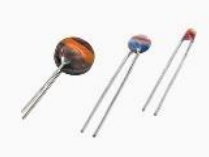
\includegraphics[scale=0.35]{introduccion/imagenes/termistores}
	\textbf{\caption{\small{Termistores \cite{dieciseis}.}}}
	\label{Seccion1.5.1:Figura1.5}
\end{figure}

\textbf{Tipos de sensores de temperatura} \\

\textbf{RTD} \\

Los RTD son sensores de temperatura que utilizan la propiedad de resistencia y coeficiente térmico de un metal (conductor), se basan en el principio de equilibrio térmico que señala que cuando un metal se encuentra en un medio que tiene mayor temperatura que él, éste tiende a aumentar su temperatura, siempre y cuando el volumen y la masa no sean mayor que el del medio con el que interactúa. Las RTD son utilizadas en el sector industrial, entre las características más destacadas es su resistencia a altas temperaturas, su alta sensibilidad, tienen una exactitud mínima de $1^{\circ}$C, tienen un tiempo de vida alto. \\

\textbf{NTC} \\

Las NTC son sensores elaborados por óxidos semiconductores que responden disminuyendo su resistencia a medida que aumenta la temperatura, son sensores con alta sensibilidad, son utilizados para monitorear que la temperatura no sobrepase un rango. \\

\textbf{PTC} \\

Las PTC son termistores con un coeficiente de temperatura positivo que al aumentar la temperatura aumenta su resistencia, son elaborados con óxidos y conductores, se utilizan para elaborar sistemas de control de temperatura, con el fin de no sobrepasar cierta temperatura ya que esta puede ser critica \cite{diecisiete}. \\

\textbf{Termopares} \\

Son sensores que se elaboran uniendo dos conductores, están basados en el principio de Seebeck y Peltier, el efecto de Seebeck dice que cuando la unión de los metales presenta diferentes temperaturas se produce un voltaje muy pequeño, que va en incremento con la temperatura, mientras que el efecto Peltier dice que transmitir una corriente en la unión de los metales se produce un flujo de calor. Los termopares se utilizan en sistemas de refrigeración para disminuir las temperaturas o aumentarlas, además de sensar la temperatura \cite{dieciocho}. \\

\textbf{Sensores a base de Circuitos Integrados} \\

Los circuitos integrados son dispositivos que están formados de elementos electrónicos, que permiten tener la misma funcionalidad que un circuito electrónico, solo que en un espacio reducido. En la actualidad tienen funciones específicas desde reguladores de voltaje, corriente hasta medir temperatura. \\

\textbf{Sensores Infrarrojos} \\

Otra de las propuestas interesantes que tenemos son los sensores de radiación térmica, estos funcionan midiendo la energía que emiten los objetos, en la región infrarroja, están construidos por un sistema óptico que enfoca el objeto, utilizando un diodo láser que ilumina la zona captando la energía desprendida de los objetos. \\

Presentan un inconveniente acorde a los materiales que presentan emisividad, que es la proporción de radiación térmica emitida por una superficie u objeto debido a su temperatura. \\

Los cuerpos negros presentan una emisividad igual a uno, en la práctica todos los cuerpos tienen esta propiedad de acuerdo a su color, los sensores de radiación vienen ajustados para una emisividad predeterminada, por lo que si se tiene otra emisividad diferente se tendrá que calibrar \cite{diecinueve}. 

\subsection{Sensor acelerómetro}
\renewcommand{\theequation}{\arabic{equation}}
\newcounter{neq}
\setcounter{equation}{\arabic{neq}}

\textbf{Definición} \\

Como ya se mencionó anteriormente, los acelerómetros son dispositivos que miden la aceleración, que es la tasa de cambio de la velocidad de un objeto y son útiles para detectar las vibraciones en los sistemas o para aplicaciones de orientación \cite{veinte}. \\

El acelerómetro calcula la aceleración por medio de la siguiente formula: \\

\begin{equation}
	\alpha = \frac{F}{m}
	\addtocounter{neq}{1}
\end{equation} \\

Dicha fórmula es la segunda ley de Newton y establece que, en un cuerpo con masa constante, la aceleración del cuerpo es proporcional a la fuerza que actúa sobre él mismo, dónde $\alpha$ es la aceleración, \textit{F} es la fuerza y \textit{m} la masa de un cuerpo. \\

La aceleración se calcula en unidades de metro por segundo al cuadrado (m/s2), o en fuerza G (g), que es aproximadamente de 9.8 m/s2. Los acelerómetros son dispositivos electromecánicos que detectan las fuerzas de aceleración, ya sea estática (incluyen gravedad) o dinámica (incluyen vibraciones y movimiento) \cite{veinte}. \\

El giroscopio se basa en el efecto Coriolis para medir la velocidad angular, el cual consiste en una masa de prueba de resonancia montada en el silicio. El giroscopio es, a diferencia de un acelerómetro, un sensor activo. La masa de prueba es empujada hacia atrás y hacia adelante por peines de conducción. Una rotación del giroscopio genera una fuerza de Coriolis que actúa sobre la masa que se traduce en un movimiento en una dirección diferente. El movimiento en esta dirección se mide mediante electrodos y representa la velocidad de giro \cite{veintiuno}. \\

El giroscopio calcula la velocidad angular por medio de la siguiente formula: \\

\begin{equation}
	\varPhi = \frac{d\theta}{dt}
	\addtocounter{neq}{1}
\end{equation} \\

Dicha fórmula establece que, la velocidad angular es la tasa de cambio del desplazamiento angular por unidad de tiempo, es decir que tan rápido gira un cuerpo alrededor de su eje y las unidades de velocidad angular son radianes por segundo (rad/s). \\

\textbf{Tipos de sensores acelerómetros \cite{veintidos}:} \\ 

\begin{itemize}
	\item \textbf{Acelerómetros mecánicos} \\
	
	Acelerómetros mecánicos, tales como el acelerómetro de masa sísmica, el sensor de velocidad, y el interruptor magnético mecánico, detectan la fuerza impuesta sobre una masa cuando se produce aceleración. La masa se resiste a la fuerza de la aceleración y de este modo provoca una deformación o un desplazamiento físico, que puede ser medido por los detectores de proximidad o galgas extensiométricas (como se muestra a continuación). Muchos de estos sensores están equipados con dispositivos de amortiguación, tales como muelles o imanes para impedir la oscilación. 
	
	\begin{figure}[h]
		\centering
		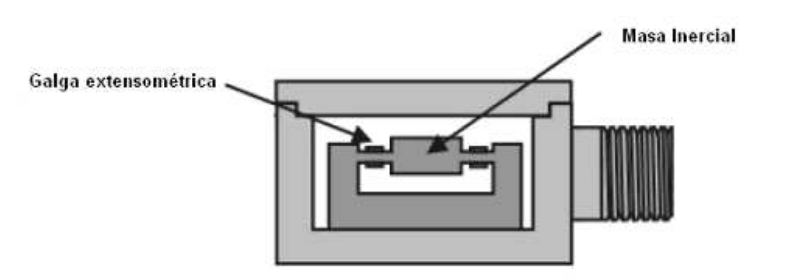
\includegraphics[scale=0.35]{introduccion/imagenes/acelerometro_mecanico}
		\textbf{\caption{\small{Acelerómetro tipo mecánico \cite{veintitres}.}}}
		\label{Seccion1.5.4:Figura1.6}
	\end{figure}

	\item \textbf{Acelerómetros Piezoeléctricos} \\
	
	Acelerómetros piezoeléctricos son ampliamente utilizados para la aceleración de propósito general, mediciones de choque y vibración. Básicamente son transductores de movimiento con grandes señales de salida y comparativamente de pequeños tamaños. Están disponibles con muy altas frecuencias naturales y son por lo tanto adecuados para aplicaciones de alta frecuencia y mediciones de choque. Estos dispositivos utilizan una masa en contacto directo con el componente piezoeléctrico, o cristal. Cuando un movimiento variable se aplica al acelerómetro, el cristal experimenta una excitación de fuerza variable, causando una carga proporcional q eléctrica a ser desarrollada a través de esta. Se clasifican en dos tipos: \\
	
	\begin{enumerate}
		\item El primero de ellos es el acelerómetro de salida de carga de alta impedancia. En este tipo de acelerómetro, el cristal piezoeléctrico genera una carga eléctrica que está conectada directamente a los instrumentos de medición. La salida de carga requiere instalaciones e instrumentación especiales, que habitualmente encontramos en los centros de investigación. Este tipo de acelerómetro también se emplea en aplicaciones de altas temperaturas $(>120^{\circ}C)$ en las que no se pueden utilizar modelos de baja impedancia. \\
		
		\item El segundo tipo de acelerómetro es el acelerómetro de salida de baja impedancia. Un acelerómetro de baja impedancia incluye un acelerómetro de carga en su extremo delantero, así como un minúsculo microcircuito integrado y un transistor FET (de efecto de campo) que convierte la carga en una tensión de baja impedancia que puede interaccionar fácilmente con la instrumentación estándar. Este tipo de acelerómetro es el que se emplea habitualmente en la industria. Una fuente de alimentación para acelerómetro como la ACC-PS1 proporciona al microcircuito un suministro eléctrico adecuado de 18 a 24 V a una corriente constante de 2 mA y elimina la corriente de polarización CC. Este tipo de fuente de alimentación suele generar una señal de salida a partir de cero de hasta +/- 5 V dependiendo del índice mV/g del acelerómetro. 
		
		\begin{figure}[h]
			\centering
			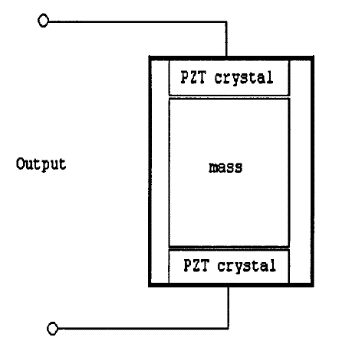
\includegraphics[scale=0.55]{introduccion/imagenes/acelerometro_piezoelectrico}
			\textbf{\caption{\small{Acelerómetro tipo piezoeléctrico \cite{veintitres}.}}}
			\label{Seccion1.5.4:Figura1.7}
		\end{figure}		
	\end{enumerate}

	\item \textbf{Acelerómetros Piezoresistivos} \\
	
	Acelerómetros piezoresistivos son esencialmente medidores de deformación de semiconductor con grandes factores de calibre factores de alto calibre se obtienen debido a que la resistividad del material depende principalmente de la tensión, no sólo en las dimensiones. El aumento de la sensibilidad es crítica en la medición de la vibración, ya que permite la miniaturización del acelerómetro. La mayoría de los acelerómetros piezorresistivos utilizan dos o cuatro calibradores activos dispuestos en un puente de Wheatstone. Se utilizan resistencias extra de precisión, como parte del circuito en serie con la entrada para controlar la sensibilidad, equilibrio y la compensación de los efectos de temperatura. En algunas aplicaciones, topes de sobrecarga son necesarios para proteger los medidores de insumos de alta amplitud. Estos instrumentos son útiles para la adquisición de información de vibración a bajas frecuencias (por ejemplo, por debajo de 1 Hz). De hecho, los sensores piezorresistivos son inherentemente verdaderos dispositivos de medición de aceleración estática. Las características típicas de acelerómetros piezorresistivos pueden ser 100 mV g-1 en la sensibilidad, 0 - 750 Hz en rango de frecuencia, 2500 Hz en la frecuencia de resonancia, 25 g en rango de amplitud, 2,000 g en índice de choque, de 0 a 95$^{\circ}$C en el rango de temperatura, con una masa total de aproximadamente 25g. Los sensores piezoresistivos operan con elementos extensométricos son sensibles a la temperatura y requieren una compensación. Se prefieren para las aplicaciones de vibraciones de baja frecuencia, descarga de larga duración, y de aceleración constante. Las unidades piezoresistivas son resistentes, y pueden operar a frecuencias de hasta 2,000 Hz. 
	
	\begin{figure}[h]
		\centering
		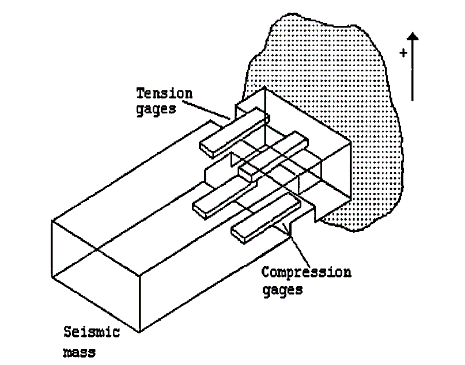
\includegraphics[scale=0.55]{introduccion/imagenes/acelerometro_piezoresistivo}
		\textbf{\caption{\small{Acelerómetro tipo piezoresistivo  \cite{veintitres}.}}}
		\label{Seccion1.5.4:Figura1.8}
	\end{figure} 

	\item \textbf{Acelerómetros capacitivos} \\
	
	Acelerómetros diferencial-capacitancia se basan en el principio del cambio de la capacitancia en proporción a la aceleración aplicada. Vienen en diferentes formas y tamaños. En un tipo, la masa sísmica del acelerómetro se hace como el elemento móvil de un oscilador. La masa sísmica se apoya en una disposición de haz paralelo de movimiento elástico de la base. El sistema se caracteriza por tener una cierta frecuencia nominal definida cuando no alterados. Si se acelera el instrumento, la frecuencia varía por encima y por debajo del valor nominal, dependiendo de la dirección de la aceleración. En acelerómetros de capacidad de detección, micro mecanizados de placas capacitivas (placas de condensador CMOS solo 60 micras de profundidad) forman una masa de unos 50 micro gramos. Como la aceleración deforma las placas, un cambio de capacitancia es medible. \\
	
	\begin{figure}[h]
		\centering
		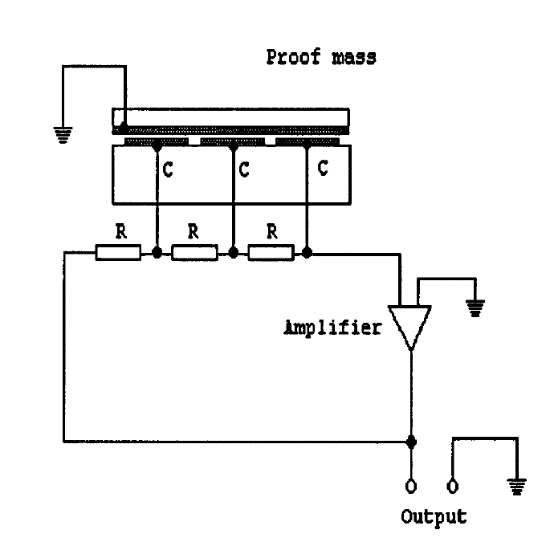
\includegraphics[scale=0.55]{introduccion/imagenes/acelerometro_capacitivo}
		\textbf{\caption{\small{Acelerómetro de capacitivo \cite{veintitres}.}}}
		\label{Seccion1.5.4:Figura1.9}
	\end{figure} 

	\item \textbf{Acelerómetro térmico} \\
	
	Estos acelerómetros hacen uso de una masa sísmica que está suspendida por un resorte o una palanca dentro de un marco rígido. El marco que lleva la masa sísmica está conectado firmemente a la fuente de vibración que tenga características medibles. Como el sistema vibra, la masa tiende a permanecer fija en su posición de modo que el movimiento puede ser registrado como un desplazamiento relativo entre la masa y el marco. Este desplazamiento es detectado por un transductor apropiado y la señal de salida se procesa adicionalmente. Sin embargo, la masa sísmica no permanece absolutamente constante; pero para frecuencias seleccionadas, de manera satisfactoria puede actuar como una posición de referencia. Mediante la selección apropiada de la masa, la primera, y combinaciones de los amortiguadores, los instrumentos sísmicos pueden ser utilizados ya sea para la aceleración o mediciones de desplazamiento. En general, una gran masa y resorte suave son apropiados para mediciones de vibración y de desplazamiento, mientras que una masa relativamente pequeña y resorte rígido se utilizan en acelerómetros. Este sensor detecta la posición a través de la transferencia de calor. Una masa sísmica se coloca encima de una fuente de calor. Si la masa se mueve a causa de la aceleración, la proximidad de la fuente de calor y la temperatura de la masa cambia. Las termopilas de polisilicio se utilizan para detectar cambios en la temperatura. 
	
	\begin{figure}[h]
		\centering
		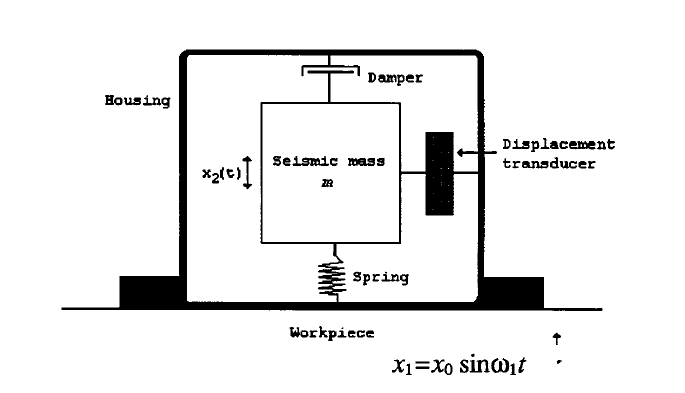
\includegraphics[scale=0.55]{introduccion/imagenes/acelerometro_termico}
		\textbf{\caption{\small{Acelerómetro térmico \cite{veintitres}.}}}
		\label{Seccion1.5.4:Figura1.10}
	\end{figure} 

	\item \textbf{Acelerómetro con tecnología MEMS} \\
	
	Estos acelerómetros son ampliamente utilizados en aplicaciones como: dinámica de vehículos, detección de orientación de teléfonos móviles, estabilidad de imagen, inclinación, detección de golpes y dispositivos antirrobo. \\
	
	Los acelerómetros de capacitancia variable están disponibles en varias configuraciones, incluidos sensores de vibraciones basados en un circuito oscilador sintonizable y sistemas mecánicos micro eléctricos (MEMS). Los circuitos de oscilador sintonizable incorporan un capacitor con una placa que actúa como una masa móvil tipo diafragma en relación con otras placas fijas. La aceleración hace que el diafragma se flexione, creando un cambio capacitivo. Esto cambia la tensión pico de la oscilación. Los acelerómetros MEM se implementan como un capacitor variable modificado por una viga en voladizo conectada a una masa de prueba. Están disponibles en dispositivos compatibles con 1 a 3 ejes. Acelerómetros MEMS utilizan interfaces seriales como I2C y SPI. Tienen alta linealidad y se utilizan mayormente en aplicaciones de baja frecuencia. 
	
	\begin{figure}[h]
		\centering
		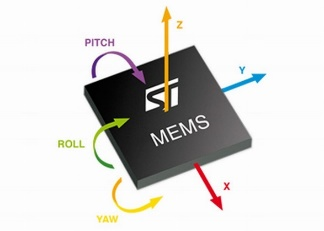
\includegraphics[scale=0.75]{introduccion/imagenes/acelerometro_MEMS}
		\textbf{\caption{\small{Acelerómetro con tecnología MEMS \cite{veinticuatro}.}}}
		\label{Seccion1.5.4:Figura1.11}
	\end{figure} 
\end{itemize}

\subsection{Sensor de frecuencia cardíaca}

\textbf{Definición} \\

La frecuencia cardíaca permite medir la cantidad de sangre por minuto que llega al corazón, por ello para determinar esa variable necesitamos un dispositivo que mida la frecuencia del corazón, por lo tanto a continuación se dará una definición del sensor para este tipo de variable, es un dispositivo conformado por un transmisor y un receptor conformados por fotodiodos, los cuales tienen la función de detectar la cantidad de sangre que fluye dependiendo de la zona donde sea colocado en un determinado tiempo. \\

\textbf{Tipos de sensores de frecuencia cardíaca} \\ 

\textbf{Óptico} \\

Emplean fotocélulas como elementos de detección. A veces disponen de un cabezal que contiene un emisor de luz y la fotocélula de detección del haz reflejado sobre el objeto. Otros trabajan en modo barrera y se utilizan para cubrir mayores distancias, con fuentes luminosas independientes del detector. Ambos tipos suelen trabajar con frecuencias en la banda de infrarrojos. Su utilización principal es como detectores de posición. El principio de funcionamiento está basado en la generación de un haz luminoso por parte de un fotoemisor, que se proyecta sobre un fotorreceptor, o bien, sobre un dispositivo reflectante. La interrupción o reflexión del haz, por parte del objeto a detectar, provoca el cambio de estado en la salida de la fotocélula. \\

Se clasifican según su sistema de detección: 

\begin{itemize}
	\item Sistema de detección de “barrera”
	\item Sistema de detección “réflex” 
	\item Sistema de detección “autoreflex”	
\end{itemize}

\textbf{Fotoeléctrico de barrera} \\

Dispone de emisor y receptor de haz luminoso dispuestos separadamente. \\

\textbf{Óptico tipo réflex} \\

Concentra en un solo bloque el emisor y receptor, siendo más fácil su instalación, aunque requiere un dispositivo reflector. Para este cometido se suele emplear un sistema catadióptrico, que tiene la propiedad del triedro trirectangular, el cual refleja la luz en la misma dirección en la que llega. Dispone de una mayor distancia de detección que el sistema de barrera, teniendo en cuenta que el trayecto que recorre el haz de luz es el doble. \\

\textbf{Óptico tipo autoreflex} \\

En este sistema es el propio objeto a detectar el que funciona como elemento reflector, lo cual simplifica la tarea de instalación. Por el contrario, su inconveniente es que dispone de una menor distancia de detección en comparación con los dos tipos anteriores. Las ventajas de este tipo de detectores son la inmunidad a perturbaciones electromagnéticas, las grandes distancias de detección, alta velocidad de respuesta, identificación de colores y detección de pequeños objetos. Una variable importante son los construidos de fibra óptica que permite separar el punto emisor y el detector de la unidad principal del sensor con las ventajas de accesibilidad que ello proporciona \cite{veinticinco}. \\

\textbf{Tecnología fotopletismografía} \\

La fotopletismografía está basada en la medida y análisis de una señal óptica relacionada con los cambios en el volumen sanguíneo, que permite medir la componente pulsátil del latido del corazón y evaluar así la circulación sanguínea Esta técnica es ampliamente usada en la práctica médica como parte de los pulsioxímetros, para medir el pulso, equivalente al ritmo cardíaco, y la saturación de oxígeno, o relación entre la concentración de hemoglobina oxigenada y la concentración total de hemoglobina, habitualmente en la punta de los dedos \cite{veintiseis}. \\

\textbf{Principios Físicos:} Detecta el flujo de sangre cutáneo y traduce sus pulsaciones. Consiste en la emisión de luz infrarroja desde un diodo emisor y un fotodetector adyacente que recibe la luz infrarroja reflejada. A medida que aumenta el flujo de sangre cutáneo aumenta la cantidad de luz reflejada. De esta manera obtenemos una medida cualitativa del flujo sanguíneo cutáneo. Se utiliza preferentemente en la medición de la presión digital. \\

\textbf{Oxímetros} \\

La oximetría de pulso es un método no invasivo que permite la estimación de la saturación de oxígeno de la hemoglobina arterial y también vigila la frecuencia cardiaca y la amplitud del pulso \cite{veintisiete}. \\

Para la determinación de la saturación de hemoglobina arterial con oxígeno (SpO2), el oxímetro de pulso o pulsioxímetro usa la espectrofotometría basada en que la oxihemoglobina u hemoglobina oxigenada (HbO2) y la desoxihemoglobina o hemoglobina reducida (Hb) absorben y transmiten determinadas longitudes de onda del espectro luminoso para la luz roja (640-660nm) y la luz infrarroja (910-940nm). La HbO2 absorbe más la luz infrarroja y permite el paso de la luz roja; por el contrario, la Hb absorbe más la luz roja (R) y permite el paso de la luz infrarroja (IR). El radio de la absorción de la luz R e IR mide el grado de oxigenación de la hemoglobina. \\

Los oxímetros de pulso tienen dos sensores o sondas con diodos emisores de luz (LED), uno para luz IR y otro para la R, además, de un fotodiodo detector. Para medir el oxígeno los LED y el fotodiodo detector deben ponerse en puntos opuestos dejando en medio el tejido translucido (pulpejo del dedo, pabellón auricular, etc). El mecanismo que permite la lectura de la oxigenación es que en cada pulsación de la sangre arterial se transmiten valores lumínicos, detectando al mismo tiempo la frecuencia cardíaca \cite{veintiocho}. 

\subsection{Microcontroladores}

En la actualidad el uso de microcontroladores es indispensable para desarrollar aplicaciones dedicadas, debido a que contienen una variedad de módulos que nos permiten interactuar con el mundo físico en tiempo real. A continuación, definiremos los conceptos teóricos que utilizaremos en la elaboración del proyecto, dando una noción de la utilidad que nos aporta un microcontrolador. Antes de mencionar a los microcontroladores es necesario mencionar que es un microprocesador ya que es su antecesor. \\

El microprocesador es un circuito integrado que contiene solo la unidad central de procesamiento (CPU), es utilizado para procesar grandes volúmenes de información, para ser utilizados es necesario conectar dispositivos periféricos.
En el siguiente apartado tenemos algunas definiciones de microcontrolador. \\

Es un circuito integrado o chip que incluye en su interior las tres unidades funcionales de un computador: CPU, memoria y unidades de entrada y salida, pero con capacidades limitadas y un alto nivel de especialización. \\

Lo definimos como un dispositivo dedicado, que en su memoria sólo reside un programa destinado que permite controlar una aplicación determinada, sus unidades de entrada y salida soportan la conexión de sensores y dispositivos de control que permitan efectuar el proceso deseado. Es un microprocesador optimizado, utilizado para controlar equipos electrónicos, diseño de sistemas de comunicación, monitoreo y adquisición de señales físicas, procesamiento de señales analógicas y digitales. \\

El microcontrolador es un circuito integrado de alta escala de integración que incorpora una CPU, memorias, dispositivos de entrada y salida. \\

La diferencia que hay entre un microcontrolador y un microprocesador, el microprocesador solo contiene la CPU mientras que el microcontrolador contiene una CPU, memorias y dispositivos que interactúan con el exterior, es la razón por la que los microcontroladores no han remplazado a los microprocesadores, es que los microprocesadores se concentran en el procesamiento de información y cálculos, y los microcontroladores se utilizan en aplicaciones personalizadas de tiempo real \cite{veintinueve}. 

\begin{figure}[h]
	\centering
	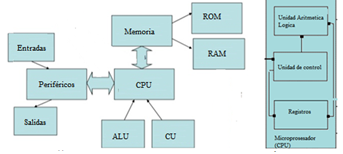
\includegraphics[scale=0.75]{introduccion/imagenes/microcontrolador}
	\textbf{\caption{\small{Diagramas de un microcontrolador (lado izquierdo) y microprocesador (lado derecho)  \cite{veintinueve}.}}}
	\label{Seccion1.5.5:Figura1.12}
\end{figure} 

La idea de utilizar microcontroladores es la tener un módulo específico que se concentre en una tarea repetitiva y de alguna manera dividir el trabajo. 

\begin{figure}[h]
	\centering
	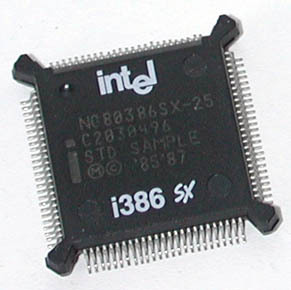
\includegraphics[scale=0.35]{introduccion/imagenes/microprocesador}
	\textbf{\caption{\small{Microprocesador \cite{treinta}.}}}
	\label{Seccion1.5.5:Figura1.13}
\end{figure} 

En la Tabla 1.3 se da la clasificación general de los microcontroladores de acuerdo a sus características principales. \\

	\begin{table}
	\centering
		\begin{tabular}{|p{4cm}|p{7.5cm}|}
			\hline
			Clasificación de los microcontroladores por & Descripción \\
			\hline \hline
			Tamaño de los datos	& 4 bits, 8 bits, 16 bits, 32 bits, 64 bits \\
			\hline
			Arquitectura interna & Von Neumann, Harvard \\
			\hline
			Arquitectura del procesador & CISC (Computador de juego de instrucciones complejo) RISC (Computador de juego de instrucciones reducido) \\		
			\hline
		\end{tabular}
	\textbf{\caption{\small{\textbf{Clasificación de microcontroladores \cite{veintinueve}.}}}}
\end{table}

\textbf{Arquitectura interna de un microcontrolador} \\

Todos los microcontroladores en la actualidad posen dos modelos básicos de arquitectura, denominadas Harvard y Von Neumann, estas arquitecturas tienen diferentes formas de intercambiar los datos \cite{veintinueve}. \\

\begin{itemize}
	\item \textbf{Arquitectura de Von Neumann} \\
	
	Es la arquitectura tradicional de computadoras y microprocesadores, en la cual la CPU está conectada en una memoria única donde se guardan las instrucciones de programas y datos. Los microcontroladores que tienen esta arquitectura internamente soló tienen un bloque de memoria y un bus de datos de 8 bits, los datos se transmiten por este bus llegando a sobrecargarlo ocasionando que la comunicación sea lenta, por otra parte solo permite lectura o escritura de la memoria en cada pulso de reloj. 
	
	\begin{figure}[h]
		\centering
		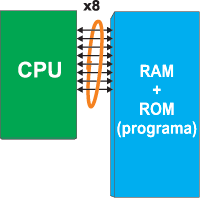
\includegraphics[scale=0.75]{introduccion/imagenes/arquitectura_von}
		\textbf{\caption{\small{Arquitectura Von Neumann \cite{treinta}.}}}
		\label{Seccion1.5.6:Figura1.14}
	\end{figure} 

	\item \textbf{Arquitectura Harvard} \\
	
	Esta arquitectura tiene la CPU conectada a dos memorias (una con las instrucciones y otra con los datos) por medio de dos buses diferentes. Una de las memorias contiene solamente las instrucciones del programa (memoria del programa) y el otro solo almacena los datos (memoria de datos). Ambos buses son totalmente independientes y pueden ser independientes y distintos anchos \cite{treintayuno}. \\
	
	\begin{figure}[h]
		\centering
		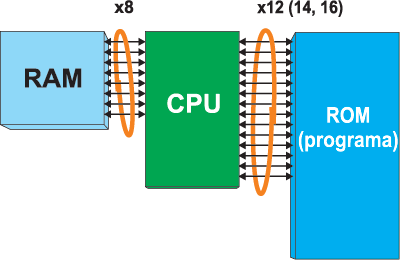
\includegraphics[scale=0.75]{introduccion/imagenes/arquitectura_harvard}
		\textbf{\caption{\small{Arquitectura Harvard \cite{treintayuno}.}}}
		\label{Seccion1.5.6:Figura1.15}
	\end{figure} 

Al tener un bus dedicado a los datos y otro a la memoria del programa, permite que la CPU pueda leer y escribir una instrucción en el mismo pulso de reloj. \\

\end{itemize}

\textbf{Juego de instrucciones} \\

Es el nombre colectivo de todas las instrucciones que tiene un microcontrolador, son instrucciones a nivel máquina que indican al microcontrolador las tareas que debe realizar, cada fabricante personaliza el número de instrucciones que maneja su microcontrolador. \\

\begin{figure}[h]
	\centering
	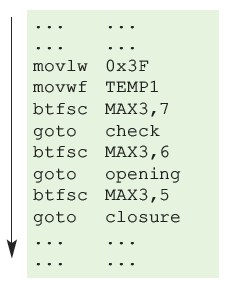
\includegraphics[scale=0.75]{introduccion/imagenes/juego_instrucciones}
	\textbf{\caption{\small{Juego de instrucciones  \cite{treintayuno}.}}}
	\label{Seccion1.5.6:Figura1.16}
\end{figure}

\textbf{Tipos de arquitectura de procesadores} \\

Los microprocesadores basados en una arquitectura CISC disponen de más de 200 instrucciones máquina, siendo estas muy complejas llegando a necesitar más de un ciclo de reloj. La ventaja de tener un juego de instrucciones complejo, es disminuir el tiempo al realizar más de una operación pues éstas en ocasiones se realizan con una sola instrucción. \\

En cuanto a los microprocesadores que utilizan la arquitectura RISC, reconoce y ejecuta pocas instrucciones básicas y realiza operaciones complejas combinando sus instrucciones, cuando se corre una instrucción regularmente solo utiliza un ciclo de reloj, por otra parte, al tener un set de instrucciones más pequeños, ayudan a optimizar los recursos de hardware de un microcontrolador \cite{veintinueve}. 

\subsection{Aplicación Móvil}

Sabemos que la era tecnológica va en aumento y la velocidad con la que evolucionan los dispositivos móviles como lo son: teléfonos celulares, tabletas y Asistentes Personales Digitales (PDA) es cada vez mayor, este impacto tiene su procedencia debido a que la población en su mayoría cuenta con un teléfono celular. \\

El estudio realizado por el Instituto Nacional de Estadística y Geografía (INEGI) en el documento: “ESTADÍSTICAS A PROPÓSITO DEL DÍA MUNDIAL DE INTERNET (17 DE MAYO)”, revela que 77.7 millones de personas usan celular y dos de cada tres usuarios cuentan con un teléfono inteligente (Smartphone), como se muestra en la figura 1.17.

\begin{figure}[h]
	\centering
	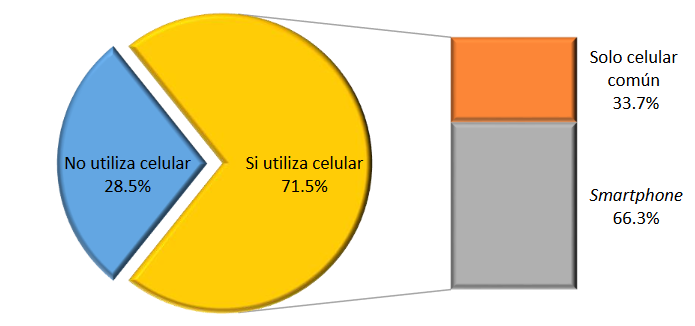
\includegraphics[scale=0.55]{introduccion/imagenes/poblacion}
	\textbf{\caption{\small{Población según condición de uso de celular, por tipo de equipo, 2015($\%$) \cite{treintayuno}.}}}
	\label{Seccion1.5.7:Figura1.17}
\end{figure}

Una aplicación móvil, es un diseño, desarrollo e implementación de un servicio que está pensado para resolver alguna problemática, dicha aplicación se ejecuta en la red y proporciona un valor añadido al cliente. En este escenario el servicio móvil necesita de dos partes: un proveedor de servicios y el usuario del servicio \cite{treintaydos}. \\

Existen dos tipos de aplicaciones móviles: \\
 \begin{itemize}
 	\item \textbf{Aplicaciones móviles web} \\
 	
 	Una aplicación web para móviles, es una aplicación web con formato para teléfonos inteligentes y tabletas, y se accede a través del navegador web del dispositivo móvil. \\
 	
 	\item \textbf{Aplicaciones móviles nativas} \\
 	
 	Una aplicación móvil nativa está construida específicamente para un dispositivo en particular y su sistema operativo. A diferencia de una aplicación web que se accede a través de Internet, una aplicación nativa se descarga desde una tienda virtual y se instala en el dispositivo. \\
 	
 	El desarrollo nativo es el desarrollo de aplicaciones que utilizan las especificaciones de los proveedores del sistema operativo (Google para Android y Apple para IOS) esto implica ajustarse a los lenguajes, frameworks e IDE’s del fabricante o proveedor \cite{treintaytres}.
 	
 \end{itemize}

	   \section{Justificación}


    \chapter{Marco Teórico } %CAP\'ITULO 2
 texto de introducción al marco teórico
	   \section{Subtema 1}


	   \section{Subtema 1}




\end{document}
%%%%%%%%%%%%%%%%%%%%%%%%%%%%%%%%%%%%%%%
%%%%%%%    FIN DEL DOCUMENTO    %%%%%%%
%%%%%%%%%%%%%%%%%%%%%%%%%%%%%%%%%%%%%%%
